%-------------------------------------------------------------------------------
\section{Prototype Design}
%-------------------------------------------------------------------------------
\label{sec:proto}

\begin{figure}[t!]
    \centering
    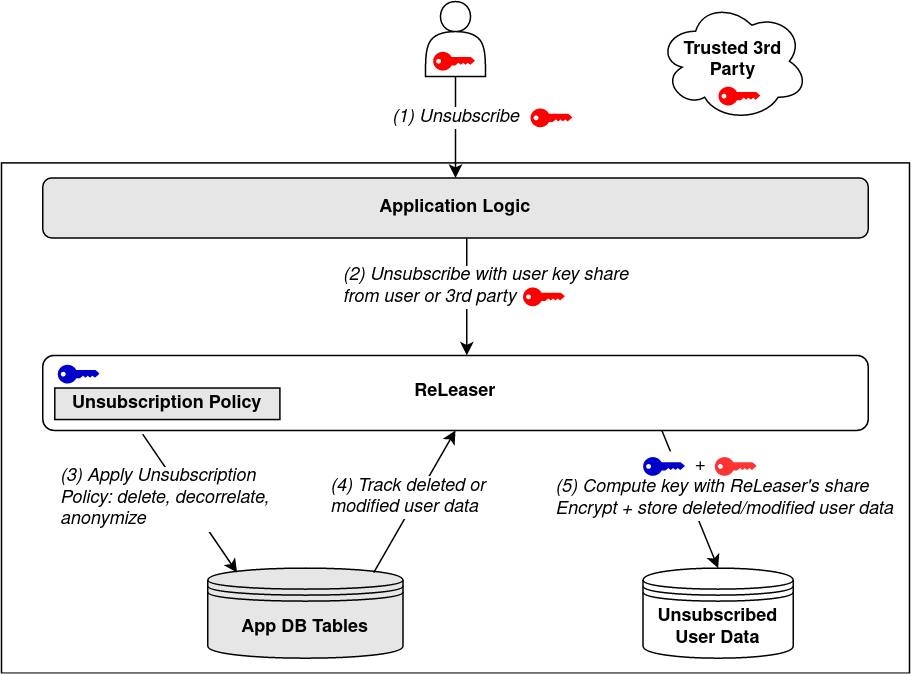
\includegraphics[width=0.5\textwidth]{img/releaser_arch}

    \caption{High-level \sys architecture. Developers specify grayed-out components.}
    \label{fig:arch}
\end{figure}

As shown in Figure~\ref{fig:arch}, \sys sits between the application logic and its database. \sys
models the application schema as an entity graph, and systematically applies the specified
unsubscription policy transformations during unsubscription.
\sys records these unsubscription transformations, and encrypts and stores this
log in an additional table. The encrypting key is secret-shared~\cite{secretsharing} among the user,
\sys, and a trusted third party so that the user can retrieve a lost key without trusting the
application or \sys. To resubscribe, \sys decrypts this log and reverses the transformations,
restoring the user's data to its original state.

\sys consists of 5K LoC of Rust, and supports SQL queries as well as \texttt{UNSUBSCRIBE
[user]} and \texttt{RESUBSCRIBE [user]} queries.
We show that \sys performs reasonably (Section~\ref{sec:perf}), and we plan to support eventually
consistent, crash-recoverable unsubscription and resubscription, sharding, and multicore parallelism.

%To amortize the cost of unsubscription and resubscription, \name preemptively creates, stores, and
%links ghost parent entities to child entities if an update creates an edge that may be decorrelated.
%\name builds in-memory materialized views on top of the underlying database, exposing ghost
%entities only if the true entity has been decorrelated, and real entities otherwise. Updates
%propagate to the materialized views when the underlying database is updated. \name answers
%application queries using these materialized views, hiding the complexity of ghost entity and
%decorrelation management.


